
%% bare_conf.tex
%% V1.3
%% 2007/01/11
%% by Michael Shell
%% See:
%% http://www.michaelshell.org/
%% for current contact information.
%%
%% This is a skeleton file demonstrating the use of IEEEtran.cls
%% (requires IEEEtran.cls version 1.7 or later) with an IEEE conference paper.
%%
%% Support sites:
%% http://www.michaelshell.org/tex/ieeetran/
%% http://www.ctan.org/tex-archive/macros/latex/contrib/IEEEtran/
%% and
%% http://www.ieee.org/

%%*************************************************************************
%% Legal Notice:
%% This code is offered as-is without any warranty either expressed or
%% implied; without even the implied warranty of MERCHANTABILITY or
%% FITNESS FOR A PARTICULAR PURPOSE! 
%% User assumes all risk.
%% In no event shall IEEE or any contributor to this code be liable for
%% any damages or losses, including, but not limited to, incidental,
%% consequential, or any other damages, resulting from the use or misuse
%% of any information contained here.
%%
%% All comments are the opinions of their respective authors and are not
%% necessarily endorsed by the IEEE.
%%
%% This work is distributed under the LaTeX Project Public License (LPPL)
%% ( http://www.latex-project.org/ ) version 1.3, and may be freely used,
%% distributed and modified. A copy of the LPPL, version 1.3, is included
%% in the base LaTeX documentation of all distributions of LaTeX released
%% 2003/12/01 or later.
%% Retain all contribution notices and credits.
%% ** Modified files should be clearly indicated as such, including  **
%% ** renaming them and changing author support contact information. **
%%
%% File list of work: IEEEtran.cls, IEEEtran_HOWTO.pdf, bare_adv.tex,
%%                    bare_conf.tex, bare_jrnl.tex, bare_jrnl_compsoc.tex
%%*************************************************************************

% *** Authors should verify (and, if needed, correct) their LaTeX system  ***
% *** with the testflow diagnostic prior to trusting their LaTeX platform ***
% *** with production work. IEEE's font choices can trigger bugs that do  ***
% *** not appear when using other class files.                            ***
% The testflow support page is at:
% http://www.michaelshell.org/tex/testflow/



% Note that the a4paper option is mainly intended so that authors in
% countries using A4 can easily print to A4 and see how their papers will
% look in print - the typesetting of the document will not typically be
% affected with changes in paper size (but the bottom and side margins will).
% Use the testflow package mentioned above to verify correct handling of
% both paper sizes by the user's LaTeX system.
%
% Also note that the "draftcls" or "draftclsnofoot", not "draft", option
% should be used if it is desired that the figures are to be displayed in
% draft mode.
%
\documentclass[conference, compsoc]{IEEEtran}
% Add the compsoc option for Computer Society conferences.
%
% If IEEEtran.cls has not been installed into the LaTeX system files,
% manually specify the path to it like:
% \documentclass[conference]{../sty/IEEEtran}





% Some very useful LaTeX packages include:
% (uncomment the ones you want to load)


% *** MISC UTILITY PACKAGES ***
%
%\usepackage{ifpdf}
% Heiko Oberdiek's ifpdf.sty is very useful if you need conditional
% compilation based on whether the output is pdf or dvi.
% usage:
% \ifpdf
%   % pdf code
% \else
%   % dvi code
% \fi
% The latest version of ifpdf.sty can be obtained from:
% http://www.ctan.org/tex-archive/macros/latex/contrib/oberdiek/
% Also, note that IEEEtran.cls V1.7 and later provides a builtin
% \ifCLASSINFOpdf conditional that works the same way.
% When switching from latex to pdflatex and vice-versa, the compiler may
% have to be run twice to clear warning/error messages.






% *** CITATION PACKAGES ***
%
%\usepackage{cite}
% cite.sty was written by Donald Arseneau
% V1.6 and later of IEEEtran pre-defines the format of the cite.sty package
% \cite{} output to follow that of IEEE. Loading the cite package will
% result in citation numbers being automatically sorted and properly
% "compressed/ranged". e.g., [1], [9], [2], [7], [5], [6] without using
% cite.sty will become [1], [2], [5]--[7], [9] using cite.sty. cite.sty's
% \cite will automatically add leading space, if needed. Use cite.sty's
% noadjust option (cite.sty V3.8 and later) if you want to turn this off.
% cite.sty is already installed on most LaTeX systems. Be sure and use
% version 4.0 (2003-05-27) and later if using hyperref.sty. cite.sty does
% not currently provide for hyperlinked citations.
% The latest version can be obtained at:
% http://www.ctan.org/tex-archive/macros/latex/contrib/cite/
% The documentation is contained in the cite.sty file itself.




% *** GRAPHICS RELATED PACKAGES ***
%
\ifCLASSINFOpdf
   \usepackage[pdftex]{graphicx}
  % declare the path(s) where your graphic files are
   \graphicspath{{../pdf/}{../jpeg/}}
  % and their extensions so you won't have to specify these with
  % every instance of \includegraphics
   \DeclareGraphicsExtensions{.pdf,.jpg,.png}
\else
  % or other class option (dvipsone, dvipdf, if not using dvips). graphicx
  % will default to the driver specified in the system graphics.cfg if no
  % driver is specified.
   \usepackage[dvips]{graphicx}
  % declare the path(s) where your graphic files are
   \graphicspath{{../eps/}{../jpeg/}}
  % and their extensions so you won't have to specify these with
  % every instance of \includegraphics
   \DeclareGraphicsExtensions{.eps, .jpg}
\fi
% graphicx was written by David Carlisle and Sebastian Rahtz. It is
% required if you want graphics, photos, etc. graphicx.sty is already
% installed on most LaTeX systems. The latest version and documentation can
% be obtained at: 
% http://www.ctan.org/tex-archive/macros/latex/required/graphics/
% Another good source of documentation is "Using Imported Graphics in
% LaTeX2e" by Keith Reckdahl which can be found as epslatex.ps or
% epslatex.pdf at: http://www.ctan.org/tex-archive/info/
%
% latex, and pdflatex in dvi mode, support graphics in encapsulated
% postscript (.eps) format. pdflatex in pdf mode supports graphics
% in .pdf, .jpeg, .png and .mps (metapost) formats. Users should ensure
% that all non-photo figures use a vector format (.eps, .pdf, .mps) and
% not a bitmapped formats (.jpeg, .png). IEEE frowns on bitmapped formats
% which can result in "jaggedy"/blurry rendering of lines and letters as
% well as large increases in file sizes.
%
% You can find documentation about the pdfTeX application at:
% http://www.tug.org/applications/pdftex




% *** MATH PACKAGES ***
%
%\usepackage[cmex10]{amsmath}
% A popular package from the American Mathematical Society that provides
% many useful and powerful commands for dealing with mathematics. If using
% it, be sure to load this package with the cmex10 option to ensure that
% only type 1 fonts will utilized at all point sizes. Without this option,
% it is possible that some math symbols, particularly those within
% footnotes, will be rendered in bitmap form which will result in a
% document that can not be IEEE Xplore compliant!
%
% Also, note that the amsmath package sets \interdisplaylinepenalty to 10000
% thus preventing page breaks from occurring within multiline equations. Use:
%\interdisplaylinepenalty=2500
% after loading amsmath to restore such page breaks as IEEEtran.cls normally
% does. amsmath.sty is already installed on most LaTeX systems. The latest
% version and documentation can be obtained at:
% http://www.ctan.org/tex-archive/macros/latex/required/amslatex/math/





% *** SPECIALIZED LIST PACKAGES ***
%
%\usepackage{algorithmic}
% algorithmic.sty was written by Peter Williams and Rogerio Brito.
% This package provides an algorithmic environment fo describing algorithms.
% You can use the algorithmic environment in-text or within a figure
% environment to provide for a floating algorithm. Do NOT use the algorithm
% floating environment provided by algorithm.sty (by the same authors) or
% algorithm2e.sty (by Christophe Fiorio) as IEEE does not use dedicated
% algorithm float types and packages that provide these will not provide
% correct IEEE style captions. The latest version and documentation of
% algorithmic.sty can be obtained at:
% http://www.ctan.org/tex-archive/macros/latex/contrib/algorithms/
% There is also a support site at:
% http://algorithms.berlios.de/index.html
% Also of interest may be the (relatively newer and more customizable)
% algorithmicx.sty package by Szasz Janos:
% http://www.ctan.org/tex-archive/macros/latex/contrib/algorithmicx/




% *** ALIGNMENT PACKAGES ***
%
%\usepackage{array}
% Frank Mittelbach's and David Carlisle's array.sty patches and improves
% the standard LaTeX2e array and tabular environments to provide better
% appearance and additional user controls. As the default LaTeX2e table
% generation code is lacking to the point of almost being broken with
% respect to the quality of the end results, all users are strongly
% advised to use an enhanced (at the very least that provided by array.sty)
% set of table tools. array.sty is already installed on most systems. The
% latest version and documentation can be obtained at:
% http://www.ctan.org/tex-archive/macros/latex/required/tools/


%\usepackage{mdwmath}
%\usepackage{mdwtab}
% Also highly recommended is Mark Wooding's extremely powerful MDW tools,
% especially mdwmath.sty and mdwtab.sty which are used to format equations
% and tables, respectively. The MDWtools set is already installed on most
% LaTeX systems. The lastest version and documentation is available at:
% http://www.ctan.org/tex-archive/macros/latex/contrib/mdwtools/


% IEEEtran contains the IEEEeqnarray family of commands that can be used to
% generate multiline equations as well as matrices, tables, etc., of high
% quality.


%\usepackage{eqparbox}
% Also of notable interest is Scott Pakin's eqparbox package for creating
% (automatically sized) equal width boxes - aka "natural width parboxes".
% Available at:
% http://www.ctan.org/tex-archive/macros/latex/contrib/eqparbox/





% *** SUBFIGURE PACKAGES ***
%\usepackage[tight,footnotesize]{subfigure}
% subfigure.sty was written by Steven Douglas Cochran. This package makes it
% easy to put subfigures in your figures. e.g., "Figure 1a and 1b". For IEEE
% work, it is a good idea to load it with the tight package option to reduce
% the amount of white space around the subfigures. subfigure.sty is already
% installed on most LaTeX systems. The latest version and documentation can
% be obtained at:
% http://www.ctan.org/tex-archive/obsolete/macros/latex/contrib/subfigure/
% subfigure.sty has been superceeded by subfig.sty.



%\usepackage[caption=false]{caption}
%\usepackage[font=footnotesize]{subfig}
% subfig.sty, also written by Steven Douglas Cochran, is the modern
% replacement for subfigure.sty. However, subfig.sty requires and
% automatically loads Axel Sommerfeldt's caption.sty which will override
% IEEEtran.cls handling of captions and this will result in nonIEEE style
% figure/table captions. To prevent this problem, be sure and preload
% caption.sty with its "caption=false" package option. This is will preserve
% IEEEtran.cls handing of captions. Version 1.3 (2005/06/28) and later 
% (recommended due to many improvements over 1.2) of subfig.sty supports
% the caption=false option directly:
%\usepackage[caption=false,font=footnotesize]{subfig}
%
% The latest version and documentation can be obtained at:
% http://www.ctan.org/tex-archive/macros/latex/contrib/subfig/
% The latest version and documentation of caption.sty can be obtained at:
% http://www.ctan.org/tex-archive/macros/latex/contrib/caption/




% *** FLOAT PACKAGES ***
%
%\usepackage{fixltx2e}
% fixltx2e, the successor to the earlier fix2col.sty, was written by
% Frank Mittelbach and David Carlisle. This package corrects a few problems
% in the LaTeX2e kernel, the most notable of which is that in current
% LaTeX2e releases, the ordering of single and double column floats is not
% guaranteed to be preserved. Thus, an unpatched LaTeX2e can allow a
% single column figure to be placed prior to an earlier double column
% figure. The latest version and documentation can be found at:
% http://www.ctan.org/tex-archive/macros/latex/base/



%\usepackage{stfloats}
% stfloats.sty was written by Sigitas Tolusis. This package gives LaTeX2e
% the ability to do double column floats at the bottom of the page as well
% as the top. (e.g., "\begin{figure*}[!b]" is not normally possible in
% LaTeX2e). It also provides a command:
%\fnbelowfloat
% to enable the placement of footnotes below bottom floats (the standard
% LaTeX2e kernel puts them above bottom floats). This is an invasive package
% which rewrites many portions of the LaTeX2e float routines. It may not work
% with other packages that modify the LaTeX2e float routines. The latest
% version and documentation can be obtained at:
% http://www.ctan.org/tex-archive/macros/latex/contrib/sttools/
% Documentation is contained in the stfloats.sty comments as well as in the
% presfull.pdf file. Do not use the stfloats baselinefloat ability as IEEE
% does not allow \baselineskip to stretch. Authors submitting work to the
% IEEE should note that IEEE rarely uses double column equations and
% that authors should try to avoid such use. Do not be tempted to use the
% cuted.sty or midfloat.sty packages (also by Sigitas Tolusis) as IEEE does
% not format its papers in such ways.





% *** PDF, URL AND HYPERLINK PACKAGES ***
%
%\usepackage{url}
% url.sty was written by Donald Arseneau. It provides better support for
% handling and breaking URLs. url.sty is already installed on most LaTeX
% systems. The latest version can be obtained at:
% http://www.ctan.org/tex-archive/macros/latex/contrib/misc/
% Read the url.sty source comments for usage information. Basically,
% \url{my_url_here}.



% *** Do not adjust lengths that control margins, column widths, etc. ***
% *** Do not use packages that alter fonts (such as pslatex).         ***
% There should be no need to do such things with IEEEtran.cls V1.6 and later.
% (Unless specifically asked to do so by the journal or conference you plan
% to submit to, of course. )


% correct bad hyphenation here
\hyphenation{op-tical net-works semi-conduc-tor}



\begin{document}
%
% paper title
% can use linebreaks \\ within to get better formatting as desired
\title{A Review of Information Security Ontology}


% author names and affiliations
% use a multiple column layout for up to two different
% affiliations

\author{Wan Nor Azura bt. Kamarudin\\Fakulti Teknologi dan Sains Maklumat\\Universiti Kebangsaan Malaysia
\\Email: azurawn@yahoo.com\\Matrix No: P47925}
%\and
%\IEEEauthorblockN{Authors Name/s per 2nd Affiliation (Author)}
%\IEEEauthorblockA{line 1 (of Affiliation): dept. name of %organization\\
%line 2: name of organization, acronyms acceptable\\
%line 3: City, Country\\
%line 4: Email: name@xyz.com}
%}

% conference papers do not typically use \thanks and this command
% is locked out in conference mode. If really needed, such as for
% the acknowledgment of grants, issue a \IEEEoverridecommandlockouts
% after \documentclass

% for over three affiliations, or if they all won't fit within the width
% of the page, use this alternative format:
% 
%\author{\IEEEauthorblockN{Michael Shell\IEEEauthorrefmark{1},
%Homer Simpson\IEEEauthorrefmark{2},
%James Kirk\IEEEauthorrefmark{3}, 
%Montgomery Scott\IEEEauthorrefmark{3} and
%Eldon Tyrell\IEEEauthorrefmark{4}}
%\IEEEauthorblockA{\IEEEauthorrefmark{1}School of Electrical and Computer Engineering\\
%Georgia Institute of Technology,
%Atlanta, Georgia 30332--0250\\ Email: see http://www.michaelshell.org/contact.html}
%\IEEEauthorblockA{\IEEEauthorrefmark{2}Twentieth Century Fox, Springfield, USA\\
%Email: homer@thesimpsons.com}
%\IEEEauthorblockA{\IEEEauthorrefmark{3}Starfleet Academy, San Francisco, California 96678-2391\\
%Telephone: (800) 555--1212, Fax: (888) 555--1212}
%\IEEEauthorblockA{\IEEEauthorrefmark{4}Tyrell Inc., 123 Replicant Street, Los Angeles, California 90210--4321}}




% use for special paper notices
%\IEEEspecialpapernotice{(Invited Paper)}




% make the title area
\maketitle


\begin{abstract}
%\boldmath
The research community realize the need for a standard and formal specification of the domain Information Security in order to ensure a clear understanding amongst the researchers in different areas of the domain Information Security. Thus, the need for Information Security Ontology which has over the years evolved from merely providing domain definitions and classifications to enabling sophisticated decision-making and automation. This paper is a review of some of the work done in developing and supporting the ontology for the domain of Information Security. The review  highlights the definitions, concepts, relationships, methodologies, tools, applications and issues related to Information Security Ontology.

\end{abstract}
% IEEEtran.cls defaults to using nonbold math in the Abstract.
% This preserves the distinction between vectors and scalars. However,
% if the conference you are submitting to favors bold math in the abstract,
% then you can use LaTeX's standard command \boldmath at the very start
% of the abstract to achieve this. Many IEEE journals/conferences frown on
% math in the abstract anyway.

% no keywords




% For peer review papers, you can put extra information on the cover
% page as needed:
% \ifCLASSOPTIONpeerreview
% \begin{center} \bfseries EDICS Category: 3-BBND \end{center}
% \fi
%
% For peerreview papers, this IEEEtran command inserts a page break and
% creates the second title. It will be ignored for other modes.
\IEEEpeerreviewmaketitle



\section{Introduction}
% no \IEEEPARstart

The most basic concept in Information Security can be stated as  safeguarding of information as an asset and its confidentiality, integrity and availability. This concept and more can be specified in detail and their relations shown with the use of an ontology for Information Security. Information Security is an interesting, albeit a vast domain which include the areas of incident handling, risk assessment, cryptography and disaster recovery to name a few. These areas can be detailed further which include terms such as threats, vulnerabilities, attacks, encryption, denial of service, rootkits, virus, malicious code and many more. As is clear with these examples, their existence is acknowledged but without any relationships or classifications between them.
\\
\\
An ontology recognizes and classifies these areas and terms as concepts or classes as well as the relationships between them. The detailed description of a concept is known as its properties or slots. With the use of reasoning tools and an ontology, inferences can be made to automatically discover knowledge or solutions to support decision-making and problem-solving tasks. The Web Ontology Language (OWL) is available for developing the ontology and there are also tools available for reasoning and querying. Interestingly, ontology has its application in e-learning [3, 7], which is related to the author's current work, Learning Content Management System (LCMS) for Information Security.
\\
\\
This paper is organised as follows. The first section covers the definitions of ontology from previous works, what ontology is made up of and why it is needed in the domain of Information Security. Section two is about the methodologies used in previous works in developing an Information Security Ontology. The tools used in previous works are the focus of section three, be it tools for developing, querying or reasoning an Information Security Ontology. Section four goes further in covering the applications of ontology related to the domain of Information Security. Lastly and as a conclusion, benefits and issues related to Information Security Ontology are covered in this paper.  

% You must have at least 2 lines in the paragraph with the drop letter
% (should never be an issue)


\hfill wna
 
\hfill September 1, 2009

\subsection{What is an ontology?}
An ontology can be defined as an explicit "specification of a conceptualization", or in other words, it is explicit formal specifications of the terms in the domain and relations among them [12]. In [10] ontology is described as a highly structured system of concepts covering the processes, objects and attributes of a domain in all their pertinent complex relations. Furthermore in [3], ontology is also described as a combination of concepts, definitions and attributes organized in taxonomies [1] and extended with axioms and rules for reasoning. Nevertheless, the ultimate goal is in the way the ontology is applied to other uses in a domain, not the ontology itself [2]. For example, ontology can be applied as an enabler of automated risk assessment in the domain of Information Security. 


\subsection{The architecture of an ontology}
An ontology comprises of three major building blocks namely concepts (classes), relationships and constraints (axioms). A concept is described in detail by its properties. A concept can have sub-concepts. A concept can be linked to other concepts with "is-a" or "has-a" relationship. Properties (attributes) provide more information about a concept. They describe the internal structure and terms of a concept. Constraints are rules that model all the possible and meaningful interpretations of the concept [2, 5]. An ontology can have ontology views, as emphasised in [4] or sub-ontologies from different perspectives depending on the needs of the ontology user. Another important feature of an ontology is inheritance. Inheritance is the down-propagation of properties, with their values filled, from parents to children and further descendants [10].


\subsection{Ontology for Information Security}
Ontologies are significant in the domain of Information Security due to their role in enabling a modular approach and predicting new phenomena [10]. Ontologies represent knowledge in a standardized and formal form to enable its utilization by automated systems [6]. For example, being able to predict the types of attacks is vital in computer security incident handling. "A common language for computer security incident information" was found to be a necessity to structure the incident reports in order to enhance rapid responses [10]. Figure 1 shows the  security relationships [6] in an Information Security Ontology.
\\
\\
The use of ontologies can find its way in other areas of Information Security such as the four high-level security issues which were identified in [11]: access to Information Systems, secure communication, security management and development of secure Information Systems. The need for ontologies in the domain of Information Security is further emphasised in [13]: "What the field needs is an ontology-a set of descriptions of the most important concepts and the relationships among them. ... A great ontology will help us report incidents more effectively, share data and information across organizations, and discuss issues among ourselves. ... Maybe we can set the example by building our ontology in a machine-usable form in using XML and developing it collaboratively."

\begin{figure}[!t]
\centering
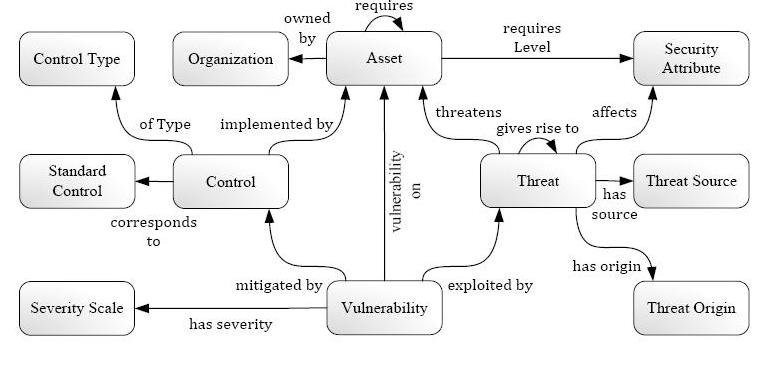
\includegraphics[width=3.0in]{sec-relationships}
% where an .eps filename suffix will be assumed under latex, 
% and a .pdf suffix will be assumed for pdflatex; or what has been declared
% via \DeclareGraphicsExtensions.
\caption{Security relationships}
\label{sec-relationships}
\end{figure}

\subsection{Methodologies for Developing Ontologies in the Domain of Information Security}
Basic approaches for developing ontologies are top-down, bottom-up and combination [2, 3, 7,]. There is no "correct" or standard method for developing ontologies [2, 7]. However, the rule-of-thumb approach can be used as a fundamental guide in the methodology for developing ontologies. [2] also stated that ontology development is an iterative process and concepts in the ontology should be close to objects and relationships in the domain of interest. Some of the methodologies used in previous works to develop Information Security Ontologies are as follows.\\
\\
In [5], the collaborative approach is used in the methodology for developing a Security Ontology. The idea used in this methodology is to build an ontology by a group of people in an iterative way, improving the ontology in every iteration. In [7], the ontology was constructed using the Description Logic (DL) knowledge engineering methodology as well as the ontology design criteria as proposed in [12]. The criteria proposed by [12] are clarity, coherence, extendibility, minimal encoding bias and minimal ontological commitment. [6] cited the ontology design criteria by [12] and stated the use of best-practice guidelines and information security standards in developing their ontology. The same ontology design criteria by [12] is also used by [9] together with the application of best practices. It is interesting to note that [9] goes a step further in contributing to the development of Information Security Ontologies by making their ontology publicly available online, downloadable and  extendible.


\subsection{Tools for Information Security Ontology}
There are many tools available for developing the ontology. Tools that have been used or proposed in previous works related to the development of Information Security Ontologies are covered next. The author has categorised the tools into three groups in this paper according to their functions for the sake of clarity.

\subsubsection{Developing and Editing the Ontology}
[2] described their experience in using Protege 2000, Ontolingua and Chimaera to edit their ontology. [5] proposed the use of Protege to populate the instances of the concepts in an ontology from the data collected. [9] used Protege and Swoop editors for their ontology. As stated in [9], Swoop is useful for finding the sources of inconsistencies in a knowledge-base.

\subsubsection{Querying the Ontology}
In [6], the SPARQL query language was used together with OWL API. [9] also used SPARQL to query and retrieve data from the ontology that they have developed. Additionally, [9] stated the advantages of using SPARQL in that it supports postprocessing, yes/no questions, sorting, filtering and string-matching. 

\subsubsection{Reasoning the Ontology}
The Pellet reasoner is used by [6] and [9] for their ontologies. As described in [6], the reasoner is used together with an editor to extract corresponding concepts and to explicitly classify them.

\begin{figure}[!t]
\centering
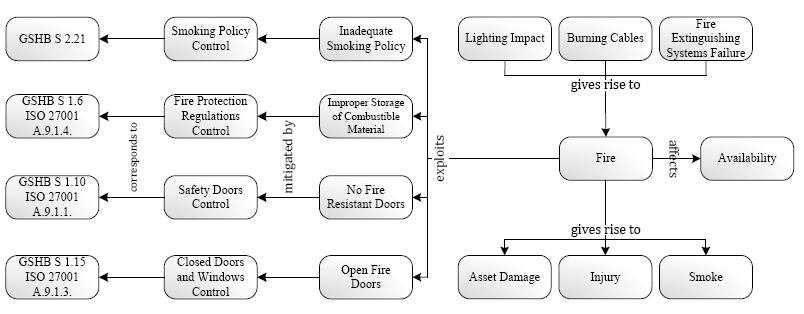
\includegraphics[width=3.0in]{fire-threat}
% where an .eps filename suffix will be assumed under latex, 
% and a .pdf suffix will be assumed for pdflatex; or what has been declared
% via \DeclareGraphicsExtensions.
\caption{Fire threat}
\label{fire-threat}
\end{figure}

\subsection{Applications of Information Security Ontology}
As mentioned previously, Information Security Ontology has many uses in its domain. Noticeably, ontology is synonym with the use of knowledge base and semantic web [4, 6] thus this makes it more significant for ontology to be applied in the domain of Information Security.
\\
\\
In [5], the Security Ontology is used together with a database of technical controls to provide customised and focused solutions in a technical level which addresses the given security requirements of a system. Information Security knowledge in the are of risk management is formalized in [6] through the use of an Information Security Ontology. As stated in [6], the ontology has been found to support a broad area of information security risk assessment. Figure 2 conceptually shows an example of the ontology from [6] applied in the risk management of a fire threat. In [8], the Information Security Ontology is applied in vulnerability analysis and management. The ontology in [8] represents knowledge for vulnerability classifications and vulnerability metrics and in a formal and structured form. As stated in [8], the ontology also enables the building of automated tools for system security. Figure 3 illustrates the vulnerability ontology in [8]. [9] comprehensively discussed the applications of their Information Security Ontology which can be used as online learning content, as a knowledge base for rule-based reasoning with semantic web applications, as a framework for further extensions and lastly as a framework to compare security products, attacks and vulnerabilities.

\begin{figure}[!t]
\centering
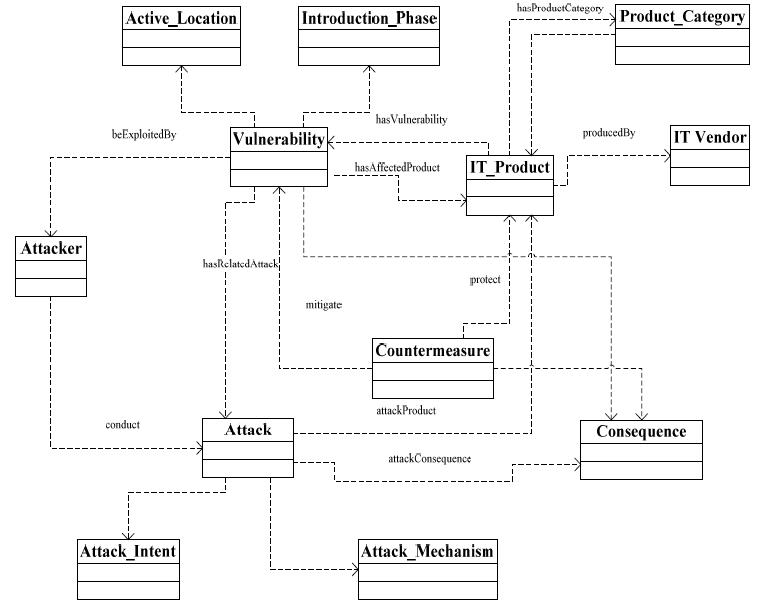
\includegraphics[width=3.0in]{ovm}
% where an .eps filename suffix will be assumed under latex, 
% and a .pdf suffix will be assumed for pdflatex; or what has been declared
% via \DeclareGraphicsExtensions.
\caption{The conceptual model of the vulnerability ontology}
\label{ovm}
\end{figure}

% An example of a floating figure using the graphicx package.
% Note that \label must occur AFTER (or within) \caption.
% For figures, \caption should occur after the \includegraphics.
% Note that IEEEtran v1.7 and later has special internal code that
% is designed to preserve the operation of \label within \caption
% even when the captionsoff option is in effect. However, because
% of issues like this, it may be the safest practice to put all your
% \label just after \caption rather than within \caption{}.
%
% Reminder: the "draftcls" or "draftclsnofoot", not "draft", class
% option should be used if it is desired that the figures are to be
% displayed while in draft mode.
%

% Note that IEEE typically puts floats only at the top, even when this
% results in a large percentage of a column being occupied by floats.


% An example of a double column floating figure using two subfigures.
% (The subfig.sty package must be loaded for this to work.)
% The subfigure \label commands are set within each subfloat command, the
% \label for the overall figure must come after \caption.
% \hfil must be used as a separator to get equal spacing.
% The subfigure.sty package works much the same way, except \subfigure is
% used instead of \subfloat.
%
%\begin{figure*}[!t]
%\centerline{\subfloat[Case I]\includegraphics[width=2.5in]%{subfigcase1}%
%\label{fig_first_case}}
%\hfil
%\subfloat[Case II]{\includegraphics[width=2.5in]{subfigcase2}%
%\label{fig_second_case}}}
%\caption{Simulation results}
%\label{fig_sim}
%\end{figure*}
%
% Note that often IEEE papers with subfigures do not employ subfigure
% captions (using the optional argument to \subfloat), but instead will
% reference/describe all of them (a), (b), etc., within the main caption.


% An example of a floating table. Note that, for IEEE style tables, the 
% \caption command should come BEFORE the table. Table text will default to
% \footnotesize as IEEE normally uses this smaller font for tables.
% The \label must come after \caption as always.
%
%\begin{table}[!t]
%% increase table row spacing, adjust to taste
%\renewcommand{\arraystretch}{1.3}
% if using array.sty, it might be a good idea to tweak the value of
% \extrarowheight as needed to properly center the text within the cells
%\caption{An Example of a Table}
%\label{table_example}
%\centering
%% Some packages, such as MDW tools, offer better commands for making tables
%% than the plain LaTeX2e tabular which is used here.
%\begin{tabular}{|c||c|}
%\hline
%One & Two\\
%\hline
%Three & Four\\
%\hline
%\end{tabular}
%\end{table}


% Note that IEEE does not put floats in the very first column - or typically
% anywhere on the first page for that matter. Also, in-text middle ("here")
% positioning is not used. Most IEEE journals/conferences use top floats
% exclusively. Note that, LaTeX2e, unlike IEEE journals/conferences, places
% footnotes above bottom floats. This can be corrected via the \fnbelowfloat
% command of the stfloats package.



\section{Conclusion}
The use of ontology in the domain of Information Security provides a standard and structured form to define and classify the terms, concepts and relationships between them in the domain. Information Security Ontology has many uses such as in the area of incident handling, risk assessment, disaster recovery and vulnerability management. Previous works on Information Security Ontology resulted in the development of improved and practical ontologies. However, more research is needed as the domain of Information Security is vast therefore there is always room for improvement and refinement of the ontologies. For example, as related with the current work of the author, there exists an opportunity for an ontological view of the domain of Information Security which can be applied in the form of a refined learning content on Information Security.

% conference papers do not normally have an appendix


% use section* for acknowledgement
\section*{Acknowledgment}


The author would like to thank Mr. Mohd Zamri Murah for his valuable advice and support in the work that was done to complete this paper. This review paper is submitted as partial requirement for the TS6234 course under the Masters of Information Technology (Management Information System) at the National University of Malaysia.

\newpage
% trigger a \newpage just before the given reference
% number - used to balance the columns on the last page
% adjust value as needed - may need to be readjusted if
% the document is modified later
\IEEEtriggeratref{8}
% The "triggered" command can be changed if desired:
%\IEEEtriggercmd{\enlargethispage{-5in}}

% references section

% can use a bibliography generated by BibTeX as a .bbl file
% BibTeX documentation can be easily obtained at:
% http://www.ctan.org/tex-archive/biblio/bibtex/contrib/doc/
% The IEEEtran BibTeX style support page is at:
% http://www.michaelshell.org/tex/ieeetran/bibtex/
%\bibliographystyle{IEEEtran}
% argument is your BibTeX string definitions and bibliography database(s)
%\bibliography{IEEEabrv,../bib/paper}
%
% <OR> manually copy in the resultant .bbl file
% set second argument of \begin to the number of references
% (used to reserve space for the reference number labels box)
\begin{thebibliography}{1}

\bibitem{IEEEhowto:savola2007towards}
Savola, R.M., \emph{Towards a Taxonomy for Information Security Metrics}, pp. 28--30.\hskip 1em plus
  0.5em minus 0.4em\relax Proceedings of the 2007 ACM workshop on Quality of protection, ACM New York, NY, USA, 2007.

\bibitem{IEEEhowto:noy2001ontology}
Noy, N.F. and McGuinness, D.L., \emph{Ontology Development 101: A Guide to Creating Your First Ontology}, pp. 01--05.\hskip 1em plus
  0.5em minus 0.4em\relax Knowledge Systems Laboratory, 2001.

\bibitem{IEEEhowto:todorova2007towards}
Todorova, K., \emph{Towards A Methodology For Ontology Development}, pp. 205.\hskip 1em plus
  0.5em minus 0.4em\relax Innovations in E-Learning, Instruction Technology, Assessment and Engineering Education, Springer, 2007.

\bibitem{IEEEhowto:rajugan2006ontology}
Rajugan, R. and Chang, E. and Dillon, T.S., \emph{Ontology Views: A Theoretical Perspective}, pp. 1814.\hskip 1em plus
  0.5em minus 0.4em\relax Lecture Notes in Computer Science, Springer, 2006.

\bibitem{IEEEhowto:tsoumas2005ontology}
Tsoumas, B. and Dritsas, S. and Gritzalis, D., \emph{An Ontology-Based Approach to Information Systems Security Management}, pp. 151.\hskip 1em plus
  0.5em minus 0.4em\relax Lecture Notes in Computer Science, Springer, 2005.

\bibitem{IEEEhowto:fenz2009formalizing}
Fenz, S. and Ekelhart, A., \emph{Formalizing Information Security Knowledge}, pp. 183--194.\hskip 1em plus
  0.5em minus 0.4em\relax Proceedings of the 4th International Symposium on Information, Computer, and Communications Security, ACM New York, NY, USA, 2009.

\bibitem{IEEEhowto:abel2004ontology}
Abel, M.H. and Benayache, A. and Lenne, D. and Moulin, C. and Barry, C. and Chaput, B., \emph{Ontology-based Organizational Memory for e-learning}, pp. 98--111.\hskip 1em plus
  0.5em minus 0.4em\relax Educational Technology \& Society, 2004.
  
\bibitem{IEEEhowto:wang-ovm}
Wang, J.A. and Guo, M., \emph{OVM: An Ontology for Vulnerability Management}.%, 3rd~ed.\hskip 1em plus
  %0.5em minus 0.4em\relax Harlow, England: Addison-Wesley, 1999.

\bibitem{IEEEhowto:herzog2009ontology}
Herzog, A. and Shahmehri, N. and Duma, C., \emph{An Ontology of Information Security}, pp. 278.\hskip 1em plus
  0.5em minus 0.4em\relax Techniques and Applications for Advanced Information Privacy and Security: Emerging Organizational, Ethical, and Human Issues, Information Science Reference, 2009.

\bibitem{IEEEhowto:raskin2001ontology}
Raskin, V. and Hempelmann, C.F. and Triezenberg, K.E. and Nirenburg, S., \emph{Ontology in Information Security: A Useful Theoretical Foundation and Methodological Tool}, pp. 53--59.\hskip 1em plus
  0.5em minus 0.4em\relax Proceedings of the 2001 workshop on New security paradigms, ACM New York, NY, USA, 2001.

\bibitem{IEEEhowto:siponen2007review}
Siponen, M.T. and Oinas-Kukkonen, H., \emph{A Review of Information Security Issues and Respective Research Contributions}, pp. 60--80.\hskip 1em plus
  0.5em minus 0.4em\relax ACM SIGMIS Database, ACM New York, NY, USA, 2007.      

\bibitem{IEEEhowto:gruber1995toward}
Gruber, T.R., \emph{Toward Principles for the Design of Ontologies Used for Knowledge Sharing}, pp. 907--928.\hskip 1em plus
  0.5em minus 0.4em\relax International Journal of Human Computer Studies, 1995.      

\bibitem{IEEEhowto:donner2003toward}
Donner, M., \emph{Toward a Security Ontology}, pp. 6--7.\hskip 1em plus
  0.5em minus 0.4em\relax IEEE Security and Privacy Magazine, 2003.
\end{thebibliography}

% that's all folks
\end{document}


